\documentclass[conference]{IEEEtran}
\usepackage[utf8]{inputenc}
\usepackage[T1]{fontenc}
\usepackage[polish]{babel}
\usepackage{graphicx}
\usepackage{amsmath}
\usepackage{cite}
\usepackage{url}
\usepackage{algorithmic}
\usepackage{algorithm}
\usepackage{booktabs}
\usepackage{float}
\usepackage{multirow}

\begin{document}

% ====================================================================
% TYTUŁ, AUTOR i NUMERACJA STRON
% ====================================================================
    
    \title{Porównanie efektywności metod przeszukiwania\\w algorytmie Podziału i Ograniczeń (Branch and Bound) dla Problemu Komiwojażera (TSP)}
    \author{
        \IEEEauthorblockN{Kacper Piekut}
        \IEEEauthorblockA{Numer albumu: 280879\\
        Wydział: W4N, Rok akademicki: 2025/2026, Semestr: 6\\
        Politechnika Wrocławska}
        }
    \maketitle
    \thispagestyle{empty}
    \pagestyle{plain}

% ====================================================================
% ABSTRAKT
% ====================================================================

    \begin{abstract}
        W niniejszym sprawozdaniu przedstawiono analizę algorytmu dokładnego Podziału i Ograniczeń (Branch and Bound/B\&B) rozwiązującego Problem Komiwojażera (TSP/ATSP). Zbadano wpływ trzech metod przeglądania przestrzeni rozwiązań: wszerz (BFS), w głąb (DFS) oraz najniższego kosztu (Lowest-Cost/Best-First), z wykorzystaniem metody redukcji macierzy kosztów. Ponadto sprawdzono wpływ zastosowania startowego Górnego Ograniczenia (UB) wyznaczonego za pomocą algorytmu heurystycznego RNN na złożoność czasową\\i pamięciową. Wyniki algorytmu B\&B skonfrontowano z osiągami algorytmu Przeglądu Zupełnego (Brute-Force).
    \end{abstract}
    \begin{IEEEkeywords}
        Problem Komiwojażera, Branch and Bound, Podział i Ograniczenia, BFS, DFS, Lowest-Cost, Złożoność Obliczeniowa, Złożoność Pamięciowa, RNN.
    \end{IEEEkeywords}

% ====================================================================
% I. WSTĘP I HIPOTEZY
% ====================================================================

    \section{Wstęp}
        \subsection{Hipotezy badawcze}
            Przed przystąpieniem do pomiarów sformułowano następujące hipotezy badawcze:
            \begin{itemize}
                \item \textbf{H1 (Kompromis czasowo-pamięciowy):} Wśród badanych metod przeglądu drzewa istnieje wyraźny kompromis: metoda Lowest-Cost (LC) minimalizuje czas obliczeń poprzez odwiedzenie sumarycznie najmniejszej liczby węzłów, natomiast metoda w głąb (DFS) charakteryzuje się mniejszym zużyciem pamięci operacyjnej.
                \item \textbf{H2 (Skalowalność pamięciowa):} Zapotrzebowanie na pamięć operacyjną w metodach BFS oraz LC rośnie wykładniczo wraz ze wzrostem wielkości grafu ($N$), podczas gdy zapotrzebowanie pamięciowe metody DFS rośnie jedynie liniowo.
                \item \textbf{H3 (Wpływ Górnego Ograniczenia):} Zastosowanie wysokiej jakości początkowego Górnego Ograniczenia (UB), wyznaczonego przez szybki algorytm heurystyczny (np. RNN), drastycznie redukuje zarówno czas obliczeń, jak i zużycie pamięci algorytmu B\&B, dzięki bardzo wczesnemu odcinaniu nieobiecujących gałęzi.
                \item \textbf{H4 (Granice metod dokładnych):} Mimo zastosowania redukcji macierzy i technik ograniczających, algorytm B\&B - z uwagi na silniową naturę problemu TSP - wciąż nie jest w stanie wyznaczyć rozwiązania optymalnego dla dużych instancji w racjonalnym czasie.
            \end{itemize}

% ====================================================================
% II. METODOLOGIA BADAŃ I ZASADA DZIAŁANIA
% ====================================================================

    \section{Metodologia Badań}
        \subsection{Środowisko testowe i dane wejściowe}
            Badania przeprowadzono na laptopie ASUS TUF Gaming F15 (procesor Intel Core i5-11400H 2.7-4.5 GHz, 16 GB RAM DDR4, dysk SSD NVMe 512 GB) pod kontrolą systemu Windows 11 Home (64-bit). Środowiskiem programistycznym był język C++ (kompilator MinGW GCC). 
            W badaniach wykorzystano dwa źródła danych:
            \begin{itemize}
                \item \textbf{Generowane losowo grafy pełne:} wygenerowano zestawy instancji symetrycznych i asymetrycznych o rozmiarach $N \in \langle 6, 14 \rangle$. Krawędzie losowano z rozkładu jednostajnego z przedziału $\langle 1, 100 \rangle$.
                \item \textbf{Biblioteka TSPLIB:} wykorzystano klasyczne instancje geograficzne oraz specjalistyczne instancje technologiczne VLSI.
            \end{itemize}
        \subsection{Opis zaimplementowanych algorytmów}
            W ramach badań nad optymalizacją procesu rozwiązywania problemu komiwojażera zaimplementowano dwa algorytmy: heurystyczny (służący jako generator Upper Bound) oraz dokładny, stanowiący główny przedmiot analizy.
            \subsubsection{Heurystyka wielokrotnego startu (Repetitive Nearest Neighbour)}
                Algorytm RNN (Algorithm 1) stanowi wielokrotne powielenie klasycznej zachłannej metody Najbliższego Sąsiada. Polega na iteracyjnym wyznaczaniu trasy, w którym na każdym kroku wybierany jest najmniej odległy (najtańszy) wierzchołek, który nie został jeszcze odwiedzony. Proces ten powtarzany jest $N$ razy, za każdym razem obierając za punkt startowy inny wierzchołek grafu. Wprowadzono dodatkowo rekurencyjną obsługę remisów odległościowych, polegającą na weryfikacji wszystkich równoznacznych ścieżek. Po zakończeniu poszukiwań zapamiętywana jest ta trasa, której całkowity koszt okazał się najmniejszy.
                \begin{algorithm}
                    \caption{Repetitive Nearest Neighbour z obsługą remisów}
                    \begin{algorithmic}[1]
                    \REQUIRE Macierz $M$ ($N \times N$), limit czasu $T$
                    \STATE $KosztOpt \leftarrow \infty$, $TrasaOpt \leftarrow \emptyset$
                    \FOR{$v = 0$ \TO $N-1$}
                        \STATE $Trasa \leftarrow \{v\}$
                        \STATE $Odw \leftarrow$ tablica \textbf{false}, $Odw[v] \leftarrow \textbf{true}$
                        \STATE $\text{Buduj}(v, Trasa, Odw)$
                        \IF{KoniecCzasu($T$)} \STATE \textbf{break} \ENDIF
                    \ENDFOR
                    \RETURN $TrasaOpt, KosztOpt$
                    \vspace{0.15cm}\hrule\vspace{0.15cm}
                    \STATE \textbf{Funkcja} $\text{Buduj}(wezel, Trasa, Odw)$
                    \IF{długość $Trasa == N$}
                        \STATE $K \leftarrow \text{Koszt}(Trasa) + M[wezel][Trasa[0]]$
                        \IF{$K < KosztOpt$}
                            \STATE $KosztOpt \leftarrow K$, $TrasaOpt \leftarrow Trasa$
                        \ENDIF
                        \RETURN
                    \ENDIF
                    \STATE $minD \leftarrow$ najkrótszy dystans do wolnego sąsiada
                    \STATE $Sasiedzi \leftarrow$ wolne wierzchołki w odl. $minD$
                    \FOR{każdego $s \in Sasiedzi$}
                        \STATE Dodaj $s$ do $Trasa$, $Odw[s] \leftarrow \textbf{true}$
                        \STATE $\text{Buduj}(s, Trasa, Odw)$
                        \STATE Usuń $s$ z $Trasa$, $Odw[s] \leftarrow \textbf{false}$
                    \ENDFOR
                    \end{algorithmic}
                \end{algorithm}
            \subsubsection{Metoda Podziału i Ograniczeń (Branch and Bound)}
                Główny przedmiot badań, zaimplementowany jako algorytm B\&B, opiera się na wyznaczaniu Dolnego Ograniczenia (LB) poprzez redukcję wierszy i kolumn macierzy odległości. Zastosowany model w sposób systematyczny dzieli przestrzeń poszukiwań i odcina gałęzie drzewa, dla których wartość LB przewyższa aktualne Górne Ograniczenie (opcjonalnie podane na wejściu z RNN). Mechanikę algorytmu sterującego przeglądem przestrzeni rozwiązań zilustrowano w Algorytmie 2. Metoda wyboru następnego węzła zależy od wariantu struktury sterującej Kolekcją (Kolejka FIFO dla BFS, Stos dla DFS oraz Kolejka Priorytetowa dla LC).
                \begin{algorithm}
                    \caption{Branch and Bound}
                    \begin{algorithmic}[1]
                    \REQUIRE Macierz $M$, pocz. $UB$, limit $T$, $Metoda$
                    \IF{$Metoda == \text{BFS}$} \STATE $Kol \leftarrow \text{Kolejka}$
                    \ELSIF{$Metoda == \text{DFS}$} \STATE $Kol \leftarrow \text{Stos}$
                    \ELSIF{$Metoda == \text{LC}$} \STATE $Kol \leftarrow \text{Kolejka Priorytetowa}$
                    \ENDIF                   
                    \STATE $KosztOpt \leftarrow UB$ (lub $\infty$)
                    \STATE $Korzen \leftarrow$ Nowy Węzeł($trasa: \{start\}, M$)
                    \STATE $Korzen.LB \leftarrow \text{Redukuj}(Korzen.M)$
                    \STATE $Kol.push(Korzen)$                    
                    \WHILE{$Kol \neq \emptyset$ \AND CzasTrwa($T$)}
                        \STATE $U \leftarrow Kol.pop()$
                        \IF{$U.LB \geq KosztOpt$} \STATE \textbf{continue} \ENDIF                        
                        \IF{$|U.trasa| == N$}
                            \STATE $KosztOpt \leftarrow U.LB$, $TrasaOpt \leftarrow U.trasa$
                            \STATE \textbf{continue}
                        \ENDIF                        
                        \FOR{nieodwiedzonego miasta $v$}
                            \STATE $V \leftarrow \text{UtworzDziecko}(U, v)$
                            \IF{$V.LB < KosztOpt$} \STATE $Kol.push(V)$ \ENDIF
                        \ENDFOR
                    \ENDWHILE
                    \RETURN $KosztOpt, TrasaOpt$                   
                    \vspace{0.15cm}\hrule\vspace{0.15cm}                   
                    \STATE \textbf{Funkcja} $\text{UtworzDziecko}(U, cel)$
                    \STATE $V \leftarrow \text{Kopiuj}(U)$, $V.trasa.push(cel)$
                    \STATE $start \leftarrow U.obecneMiasto$, $kKroku \leftarrow V.M[start][cel]$                   
                    \STATE Wiersz $start$ i kolumna $cel$ w $V.M \leftarrow \infty$
                    \STATE $V.M[cel][V.trasa[0]] \leftarrow \infty$
                    \STATE $kRed \leftarrow \text{Redukuj}(V.M)$
                    \STATE $V.LB \leftarrow U.LB + kKroku + kRed$
                    \RETURN $V$                    
                    \vspace{0.15cm}\hrule\vspace{0.15cm}
                    \STATE \textbf{Funkcja} $\text{Redukuj}(M)$
                    \STATE $koszt \leftarrow 0$
                    \FOR{wiersza $i$ w $M$}
                        \STATE $min \leftarrow \min(M[i])$ (bez $\infty$)
                        \IF{$min > 0$}
                            \STATE $M[i] \leftarrow M[i] - min$
                            \STATE $koszt \leftarrow koszt + min$
                        \ENDIF
                    \ENDFOR
                    \FOR{kolumny $j$ w $M$}
                        \STATE $min \leftarrow \min(M[j])$ (bez $\infty$)
                        \IF{$min > 0$}
                            \STATE $M[j] \leftarrow M[j] - min$
                            \STATE $koszt \leftarrow koszt + min$
                        \ENDIF
                    \ENDFOR
                    \RETURN $koszt$
                    \end{algorithmic}
                \end{algorithm}
        \subsection{Strategie przeszukiwania drzewa (BFS, DFS, LC)}
            Rozwój drzewa poszukiwań może odbywać się według różnych metod, które narzucane są bezpośrednio przez rodzaj struktury danych przechowującej nieodwiedzone węzły:
            \begin{itemize}
                \item \textbf{BFS (wszerz):} Wykorzystuje kolejkę (\textit{Queue} - FIFO). Drzewo budowane jest poziomami. Najszybciej zużywa pamięć, ponieważ przechowuje ogromne ilości węzłów pośrednich bez wczesnego schodzenia do liści.
                \item \textbf{DFS (w głąb):} Wykorzystuje stos (\textit{Stack} - LIFO). Błyskawicznie "nurkuje" na dno drzewa, szybko znajdując pierwsze pełne trasy, co sprzyja wczesnemu wyznaczaniu własnego Górnego Ograniczenia. Zużywa ułamek pamięci w stosunku do BFS.
                \item \textbf{LC (Best-First / Lowest-Cost):} Wykorzystuje kolejkę priorytetową (\textit{Priority Queue}). Węzły sortowane są rosnąco według ich wartości $LB$. Algorytm zawsze wybiera najbardziej "obiecującą" gałąź niezależnie od jej głębokości. Zazwyczaj odwiedza najmniej węzłów, ale zarządzanie kolejką narzuca dodatkowy koszt obliczeniowy na każdą operację.
            \end{itemize}
        \subsection{Konfiguracja eksperymentu}
            Wszystkie parametry badania są definiowane w zewnętrznym pliku \texttt{config.txt}, co umożliwia pełną automatyzację testów oraz szybką zmianę metod przeszukiwania drzewa bez konieczności ingerencji w kod źródłowy. Poniżej przedstawiono przykładową konfigurację:
\begin{verbatim}
ALGORITHM = DFS
GRAPH_PATH = data/tsplib/burma14.tsp
TIME_LIMIT_SECONDS = 60
REPETITIONS = 5
USE_INITIAL_UB = true
SAVE_TO_CSV = true
\end{verbatim}

% ====================================================================
% III. WYNIKI BADAŃ
% ====================================================================

    \section{Wyniki Badań}
        Wszystkie pomiary czasowe zaprezentowane w tej sekcji stanowią średnią z przeprowadzonych prób. Wartości zaprezentowano w formacie naukowym (w mikrosekundach[$\mu$s]). Zjawisko przekroczenia limitu czasu oznaczono jako \textit{TimeOut}.
        \subsection{Wpływ metod przeszukiwania oraz Górnego Ograniczenia na wydajność algorytmu B\&B}
            Na początku zbadano czasy działania poszczególnych metod na wygenerowanych grafach z pominięciem dostarczenia algorytmowi Górnego Ograniczenia ($UB = \infty$). Wyniki zebrano w Tabelach \ref{tab:czas_sym_noub} i \ref{tab:czas_asym_noub} oraz zaprezentowano na wykresach \ref{fig:wykres1} i \ref{fig:wykres2}.
            \begin{table}[H]
                \centering
                \caption{Czas B\&B [$\mu$s] w zależności od metod dla grafów symetrycznych (Bez UB)}
                \label{tab:czas_sym_noub}
                \begin{tabular}{|r|r|r|r|}
                    \hline
                    \multicolumn{1}{|c|}{$N$} & \multicolumn{1}{c|}{BFS[$\mu$s]} & \multicolumn{1}{c|}{DFS[$\mu$s]} & \multicolumn{1}{c|}{LC[$\mu$s]} \\ \hline
                    6 & $4.06\cdot10^{2}$ & $4.50\cdot10^{1}$ & $7.00\cdot10^{1}$ \\ \hline
                    8 & $2.19\cdot10^{4}$ & $3.16\cdot10^{2}$ & $2.78\cdot10^{2}$ \\ \hline
                    10 & $1.87\cdot10^{6}$ & $1.29\cdot10^{3}$ & $6.48\cdot10^{2}$ \\ \hline
                    12 & \multicolumn{1}{c|}{TimeOut} & $1.35\cdot10^{4}$ & $7.10\cdot10^{4}$ \\ \hline
                    14 & \multicolumn{1}{c|}{TimeOut} & $1.94\cdot10^{4}$ & $2.46\cdot10^{4}$ \\ \hline
                \end{tabular}
            \end{table}
            \begin{figure}[H]
                \centering
                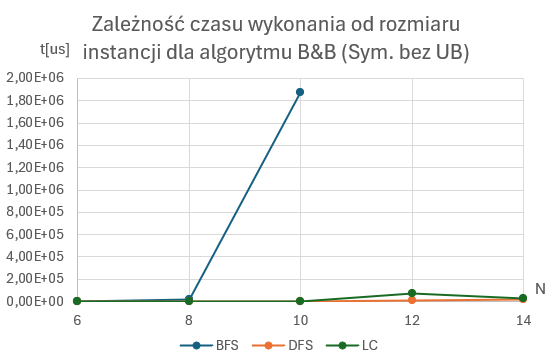
\includegraphics[width=\linewidth]{images/wykres1.png}
                \caption{Zależność czasu wykonania od rozmiaru instancji dla algorytmu B\&B (Sym. bez UB).}
                \label{fig:wykres1}
            \end{figure}
            \begin{table}[H]
                \centering
                \caption{Czas B\&B [$\mu$s] w zależności od metod dla grafów asymetrycznych (Bez UB)}
                \label{tab:czas_asym_noub}
                \begin{tabular}{|r|r|r|r|}
                    \hline
                    \multicolumn{1}{|c|}{$N$} & \multicolumn{1}{c|}{BFS[$\mu$s]} & \multicolumn{1}{c|}{DFS[$\mu$s]} & \multicolumn{1}{c|}{LC[$\mu$s]} \\ \hline
                    6 & $4.48\cdot10^{2}$ & $8.00\cdot10^{1}$ & $3.70\cdot10^{1}$ \\ \hline
                    8 & $2.17\cdot10^{4}$ & $2.21\cdot10^{2}$ & $1.11\cdot10^{2}$ \\ \hline
                    10 & $1.88\cdot10^{6}$ & $2.93\cdot10^{2}$ & $4.38\cdot10^{2}$ \\ \hline
                    12 & \multicolumn{1}{c|}{TimeOut} & $6.64\cdot10^{3}$ & $4.14\cdot10^{3}$ \\ \hline
                    14 & \multicolumn{1}{c|}{TimeOut} & $5.82\cdot10^{3}$ & $5.64\cdot10^{3}$ \\ \hline
                \end{tabular}
            \end{table}
            \begin{figure}[H]
                \centering
                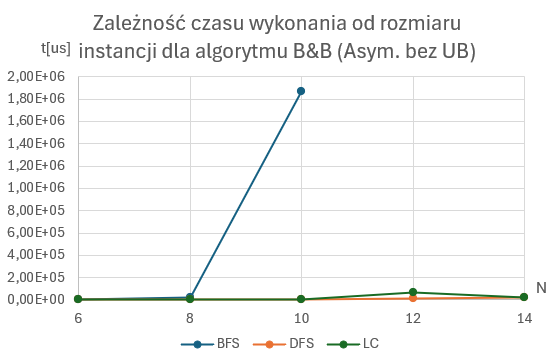
\includegraphics[width=\linewidth]{images/wykres2.png}
                \caption{Zależność czasu wykonania od rozmiaru instancji dla algorytmu B\&B (Asym. bez UB).}
                \label{fig:wykres2}
            \end{figure}
            Następnie to samo badanie powtórzono, dostarczając algorytmowi początkowe Górne Ograniczenie (UB) wyznaczone przez algorytm RNN, co obrazują Tabele \ref{tab:czas_sym_ub} i \ref{tab:czas_asym_ub} oraz Wykresy \ref{fig:wykres3} i \ref{fig:wykres5}.
            \begin{table}[H]
                \centering
                \caption{Czas B\&B [$\mu$s] w zależności od metod dla grafów symetrycznych (Z UB)}
                \label{tab:czas_sym_ub}
                \begin{tabular}{|r|r|r|r|}
                    \hline
                    \multicolumn{1}{|c|}{$N$} & \multicolumn{1}{c|}{BFS[$\mu$s]} & \multicolumn{1}{c|}{DFS[$\mu$s]} & \multicolumn{1}{c|}{LC[$\mu$s]} \\ \hline
                    6 & $2.20\cdot10^{1}$ & $2.30\cdot10^{1}$ & $2.90\cdot10^{1}$ \\ \hline
                    8 & $1.59\cdot10^{2}$ & $1.29\cdot10^{2}$ & $1.72\cdot10^{2}$ \\ \hline
                    10 & $1.48\cdot10^{3}$ & $6.89\cdot10^{2}$ & $6.42\cdot10^{2}$ \\ \hline
                    12 & $6.28\cdot10^{3}$ & $5.93\cdot10^{3}$ & $6.29\cdot10^{3}$ \\ \hline
                    14 & $2.00\cdot10^{4}$ & $1.12\cdot10^{4}$ & $1.14\cdot10^{4}$ \\ \hline
                \end{tabular}
            \end{table}
            \begin{figure}[H]
                \centering
                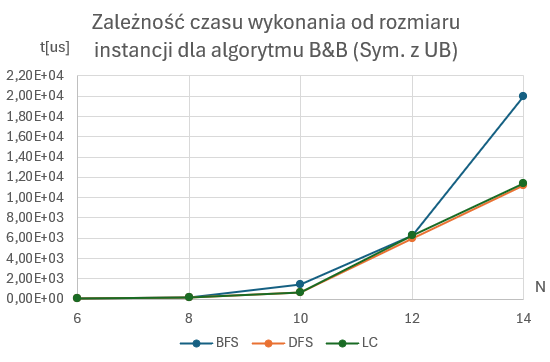
\includegraphics[width=\linewidth]{images/wykres3.png}
                \caption{Zależność czasu wykonania od rozmiaru instancji dla algorytmu B\&B (Sym. z UB).}
                \label{fig:wykres3}
            \end{figure}
            \begin{table}[H]
                \centering
                \caption{Czas B\&B [$\mu$s] w zależności od metod dla grafów asymetrycznych (Z UB)}
                \label{tab:czas_asym_ub}
                \begin{tabular}{|r|r|r|r|}
                    \hline
                    \multicolumn{1}{|c|}{$N$} & \multicolumn{1}{c|}{BFS[$\mu$s]} & \multicolumn{1}{c|}{DFS[$\mu$s]} & \multicolumn{1}{c|}{LC[$\mu$s]} \\ \hline
                    6 & $1.10\cdot10^{1}$ & $1.00\cdot10^{1}$ & $1.10\cdot10^{1}$ \\ \hline
                    8 & $6.70\cdot10^{1}$ & $7.60\cdot10^{1}$ & $6.20\cdot10^{1}$ \\ \hline
                    10 & $2.34\cdot10^{2}$ & $1.64\cdot10^{2}$ & $1.44\cdot10^{2}$ \\ \hline
                    12 & $4.02\cdot10^{3}$ & $5.18\cdot10^{2}$ & $3.34\cdot10^{2}$ \\ \hline
                    14 & $3.56\cdot10^{5}$ & $5.24\cdot10^{3}$ & $4.80\cdot10^{3}$ \\ \hline
                \end{tabular}
            \end{table}
            \begin{figure}[H]
                \centering
                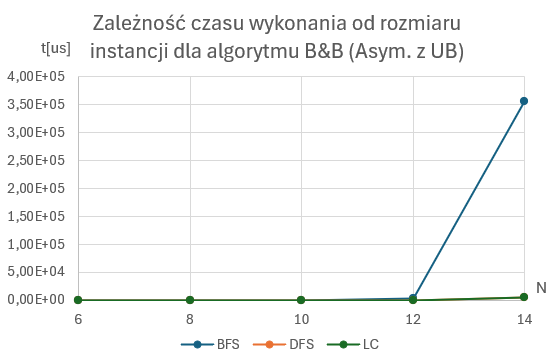
\includegraphics[width=\linewidth]{images/wykres4.png}
                \caption{Zależność czasu wykonania od rozmiaru instancji dla algorytmu B\&B (Asym. z UB).}
                \label{fig:wykres5}
            \end{figure}
            Kolejno zweryfikowano wydajność na rzeczywistych danych ze zbiorów TSPLIB. W Tabeli \ref{tab:tsplib_all} zebrano czasy metod DFS i LC. Z zestawienia całkowicie odrzucono metodę BFS z powodu niezmieszczenia się w limicie czasu.
            \begin{table}[H]
                \centering
                \caption{Czasy wykonania B\&B [$\mu$s] dla instancji TSPLIB (Z/Bez UB)}
                \label{tab:tsplib_all}
                \begin{tabular}{|c|r|r|r|r|r|}
                    \hline
                    \multicolumn{1}{|c|}{\multirow{2}{*}{Instancja}} & \multicolumn{1}{c|}{\multirow{2}{*}{$N$}} & \multicolumn{2}{c|}{Bez startowego UB} & \multicolumn{2}{c|}{Z początkowym UB} \\ \cline{3-6}
                    \multicolumn{1}{|c|}{} & \multicolumn{1}{c|}{} & \multicolumn{1}{c|}{DFS[$\mu$s]} & \multicolumn{1}{c|}{LC[$\mu$s]} & \multicolumn{1}{c|}{DFS[$\mu$s]} & \multicolumn{1}{c|}{LC[$\mu$s]} \\ \hline
                    burma14 & 14 & $2.00\cdot10^{4}$ & $4.61\cdot10^{4}$ & $2.17\cdot10^{4}$ & $4.86\cdot10^{4}$ \\ \hline
                    ulysses16 & 16 & $2.23\cdot10^{6}$ & $1.12\cdot10^{7}$ & $2.22\cdot10^{6}$ & $9.55\cdot10^{6}$ \\ \hline
                    gr17 & 17 & $6.61\cdot10^{6}$ & $2.41\cdot10^{7}$ & $5.01\cdot10^{6}$ & $6.65\cdot10^{6}$ \\ \hline
                    gr21 & 21 & $4.35\cdot10^{6}$ & $1.41\cdot10^{6}$ & $5.74\cdot10^{5}$ & $8.64\cdot10^{5}$ \\ \hline
                    ulysses22 & 22 & \multicolumn{1}{c|}{TimeOut} & \multicolumn{1}{c|}{TimeOut} & \multicolumn{1}{c|}{TimeOut} & \multicolumn{1}{c|}{TimeOut} \\ \hline
                \end{tabular}
            \end{table}
        \subsection{Porównanie B\&B z metodą Przeglądu Zupełnego (Brute-Force)}
            Aby zobrazować skalę oszczędności, jaką wnosi matematyczna redukcja macierzy, skonfrontowano wyniki czasowe dla instancji Sym. algorytmu Przeglądu Zupełnego (BF)\\z wynikami algorytmu B\&B na wykresach \ref{fig:wykres5} i \ref{fig:wykres6}.
            \begin{figure}[H]
                \centering
                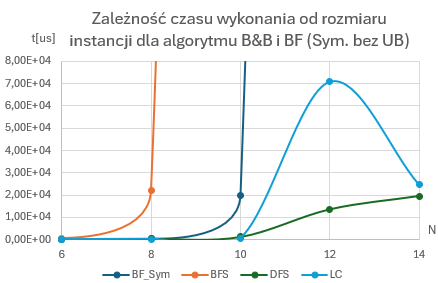
\includegraphics[width=\linewidth]{images/wykres5.png}
                \caption{Zależność czasu wykonania od rozmiaru instancji dla algorytmu B\&B i BF (Sym. bez UB).}
                \label{fig:wykres5}
            \end{figure}
            \begin{figure}[H]
                \centering
                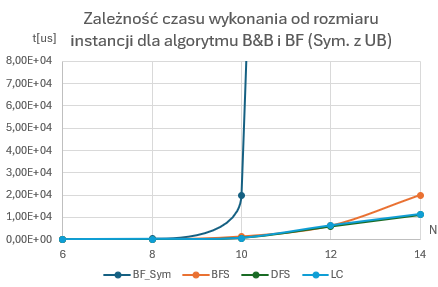
\includegraphics[width=\linewidth]{images/wykres6.png}
                \caption{Zależność czasu wykonania od rozmiaru instancji dla algorytmu B\&B i BF (Sym. z UB).}
                \label{fig:wykres6}
            \end{figure}
        \subsection{Wpływ metody przeszukiwania na złożoność pamięciową}
            Równie istotnym aspektem oceny efektywności algorytmów dokładnych, co czas obliczeń, jest ich narzut pamięciowy. Problem ten uwidacznia się zwłaszcza w metodach opartych na drzewach poszukiwań. W celu weryfikacji teoretycznych założeń zbadano maksymalną liczbę węzłów przetrzymywanych jednocześnie w strukturach takich jak kolejka, czy stos. Pomiary przeprowadzono na instancjach symetrycznych\\w wariantach bez początkowego ograniczenia (Tabela \ref{tab:pamiec_noub}) oraz z zastosowaniem początkowego UB (Tabela \ref{tab:pamiec_ub}).
            \begin{table}[H]
                \centering
                \caption{Maksymalna liczba węzłów w pamięci dla grafów Sym. (Bez UB)}
                \label{tab:pamiec_noub}
                \begin{tabular}{|r|r|r|r|}
                    \hline
                    \multicolumn{1}{|c|}{$N$} & \multicolumn{1}{c|}{BFS} & \multicolumn{1}{c|}{DFS} & \multicolumn{1}{c|}{LC} \\ \hline
                    6 & 120 & 11 & 22 \\ \hline
                    8 & 5 040 & 22 & 140 \\ \hline
                    10 & 362 880 & 37 & 233 \\ \hline
                    12 & \multicolumn{1}{c|}{TimeOut} & 56 & 4 810 \\ \hline
                    14 & \multicolumn{1}{c|}{TimeOut} & 79 & 6 344 \\ \hline
                \end{tabular}
            \end{table}
            \begin{figure}[H]
                \centering
                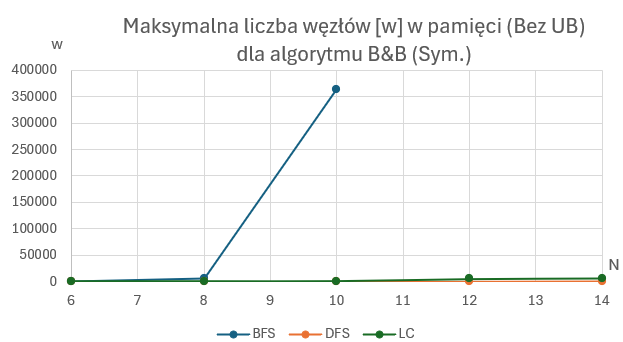
\includegraphics[width=\linewidth]{images/wykres7.png}
                \caption{Maksymalna liczba węzłów [w] w pamięci (Bez UB) dla algorytmu B\&B (Sym.).}
                \label{fig:wykres7}
            \end{figure}
            \begin{table}[H]
                \centering
                \caption{Maksymalna liczba węzłów w pamięci dla grafów Sym.\\(Z UB)}
                \label{tab:pamiec_ub}
                \begin{tabular}{|r|r|r|r|}
                    \hline
                    \multicolumn{1}{|c|}{$N$} & \multicolumn{1}{c|}{BFS} & \multicolumn{1}{c|}{DFS} & \multicolumn{1}{c|}{LC} \\ \hline
                    6 & 3 & 3 & 3 \\ \hline
                    8 & 14 & 7 & 14 \\ \hline
                    10 & 73 & 12 & 78 \\ \hline
                    12 & 212 & 25 & 319 \\ \hline
                    14 & 503 & 22 & 710 \\ \hline
                \end{tabular}
            \end{table}
            \begin{figure}[H]
                \centering
                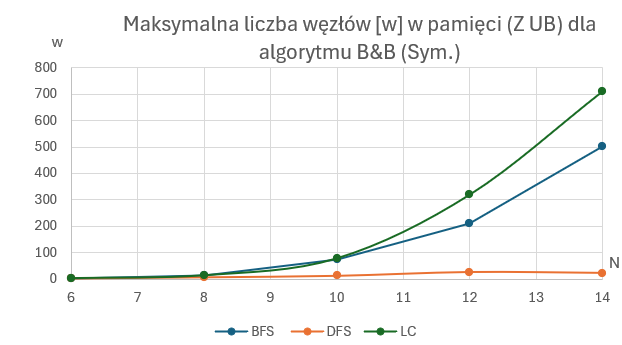
\includegraphics[width=\linewidth]{images/wykres8.png}
                \caption{Maksymalna liczba węzłów [w] w pamięci (Z UB) dla algorytmu B\&B (Sym.).}
                \label{fig:wykres8}
            \end{figure}

% ====================================================================
% IV. DYSKUSJA I WNIOSKI
% ====================================================================

    \section{Wnioski}
        Analiza przeprowadzonych badań pozwala na jednoznaczne potwierdzenie postawionych hipotez badawczych oraz sformułowanie następujących wniosków końcowych:
        \subsection{Weryfikacja hipotez i metod przeszukiwania}
            \begin{itemize}
                \item \textbf{H1 i H2 (Kompromis czasowo-pamięciowy): Potwierdzone.} Wyniki zestawione w Tabelach I--IV ukazują drastyczne różnice w zapotrzebowaniu na zasoby. Metoda BFS najszybciej osiągnęła limit czasu i pamięci, co wynika z wykładniczego przyrostu węzłów w kolejce FIFO. Metoda DFS wykazała się najwyższą efektywnością pamięciową, jednak bez wsparcia UB sprawdzała znacznie więcej węzłów niż metoda LC. Metoda LC (Lowest-Cost) zgodnie z oczekiwaniami odwiedzała najmniejszą liczbę węzłów przed znalezieniem optimum, ale zwiększyło to koszty pamięciowe.
                \item \textbf{H3 (Wpływ startowego UB): Potwierdzone.} Inicjalizacja algorytmu wartością UB wyznaczoną przez algorytm RNN skróciła czas obliczeń dla dużych instancji. Wysokiej jakości UB pozwala na drastyczne przycinanie drzewa poszukiwań już na wczesnych etapach, co jest kluczowe dla metod dokładnych.
                \item \textbf{H4 (Granice metod dokładnych): Potwierdzone.} Mimo optymalizacji, algorytm B\&B napotyka barierę wykładniczą. Dowodem jest instancja ulysses22, która mimo zastosowania najlepszych metod (DFS/LC+UB) nie została rozwiązana w limicie czasowym.
            \end{itemize}
        \subsection{Szacowanie wydajności i limitów (Nmax)}
            Maksymalny rozmiar instancji ($N_{max}$), możliwy do rozwiązania w założonym limicie czasowym, oszacowano na podstawie rzeczywistych punktów krytycznych (TimeOut) oraz trendów wzrostu zaobserwowanych w Sekcji III:
            \begin{itemize}
                \item \textbf{B\&B (BFS):} Ta metoda okazała się najbardziej ograniczona przez zasoby sprzętowe. Z Tabel I i II wynika, że stabilne wyniki uzyskiwano jedynie do $N=11$. Przy rozmiarze $N=12$ algorytm regularnie zgłaszał \textit{TimeOut}, co pozwala przyjąć \textbf{$N_{max} = 11$} dla tej metody. 
                \item \textbf{B\&B (DFS i LC):} Są to najbardziej efektywne warianty. Z Tabeli V wynika, że algorytmy te bez problemu radziły sobie z instancją \texttt{gr21} ($N=21$). Jednak bariera pojawiła się już przy $N=22$ (\texttt{ulysses22}), gdzie nastąpiło przekroczenie limitu czasu. Na tej podstawie można przyjąć, że granica wydajności dla tych metod wynosi \textbf{$N_{max} = 21$}.
            \end{itemize}
        \subsection{Charakterystyka algorytmów w kontekście efektywności}
            Na podstawie przeprowadzonych badań obu etapów (Zadanie 1 i Zadanie 2), można dokonać syntetycznej oceny przydatności algorytmów w rozwiązywaniu TSP:
            \begin{itemize}
                \item \textbf{Przegląd zupełny (Brute-Force):} Nadaje się wyłącznie do ekstremalnie małych instancji ($N < 14$). Jest nieużyteczny w praktyce, ponieważ nie posiada mechanizmów optymalizacji przeglądu.
                \item \textbf{Algorytm losowy (RAND):} Metoda o skrajnie niskiej efektywności optymalizacyjnej, generująca rozwiązania\\o ogromnym błędzie względnym. W rzeczywistej logistyce jest całkowicie bezużyteczna. Służy jako punkt odniesienia udowadniający, że inne zaimplementowane algorytmy faktycznie wykonują inteligentną optymalizację.
                \item \textbf{Heurystyki (NN, RNN):} Nadają się do bardzo dużych instancji, gdzie liczy się czas odpowiedzi, a nie idealne optimum. Algorytm RNN jest doskonałym kompromisem - pozwala uzyskać wynik bliski optymalnemu w akceptowalnym czasie. Nie nadaje się do zastosowań krytycznych, gdzie koszt trasy musi być absolutnie minimalny.
                \item \textbf{Branch and Bound (LC + UB):} Jest to najbardziej zaawansowana z badanych metod dokładnych. Nadaje się do problemów o średniej wielkości. Dzięki mechanizmowi redukcji macierzy i inteligentnemu przeszukiwaniu, potrafi znaleźć i udowodnić optimum znacznie szybciej niż Brute-Force.
                \item \textbf{Branch and Bound (DFS):} Jest to jedyna metoda dokładna, która nadaje się do systemów o bardzo ograniczonej pamięci operacyjnej, dzięki swojej liniowej złożoności pamięciowej $O(N)$.
            \end{itemize}
            \textbf{Podsumowując:} Wybór algorytmu zależy od priorytetu: jeśli kluczowa jest \textbf{gwarancja optimum}, wybieramy \textbf{B\&B LC + UB}. Jeśli kluczowa jest \textbf{szybkość przy dużym N}, jedynym wyborem są \textbf{heurystyki (RNN)}. Metody dokładne przestają być efektywne, gdy rozmiar problemu uniemożliwia zakończenie obliczeń w racjonalnym czasie.
        \section{Podsumowanie}
            Z punktu widzenia praktycznego, najlepszym kompromisem jest połączenie \textbf{metod LC (Lowest-Cost) z początkowym ograniczeniem UB z algorytmu RNN}. Taka konfiguracja najszybciej zbiega do wyniku optymalnego i potrafi udowodnić jego poprawność. W sytuacjach ekstremalnie ograniczonych zasobów pamięci RAM (np. systemy wbudowane), należy jednak skłonić się ku metod \textbf{DFS}, która mimo dłuższego czasu pracy, gwarantuje stałą, niską zajętość pamięci. Ostatecznie metoda Podziału i Ograniczeń stanowi potężne narzędzie optymalizacyjne, jednak jej zasięg ograniczony jest do małych\\i średnich instancji. Dla problemów rzeczywistych o rozmiarach $N > 30$ niezbędne staje się wykorzystanie metod metaheurystycznych.

% ====================================================================
% LITERATURA
% ====================================================================

    \begin{thebibliography}{00}
        \bibitem{vlsi_data} \textit{VLSI TSP Data}, University of Waterloo. [Online]. Dostępne: \url{https://www.math.uwaterloo.ca/tsp/vlsi/index.html}
        \bibitem{mecalux} Mecalux, \textit{Problem komiwojażera w logistyce}. [Online]. Dostępne: \url{https://www.mecalux.pl/blog/problem-komiwojazera}
        \bibitem{rudy_zto} J. Rudy, \textit{Złożoność obliczeniowa i algorytmy - Materiały pomocnicze}, PWr. [Online]. Dostępne: \url{https://kam.pwr.edu.pl/jaroslaw-rudypwr-edu-pl/files/zto/lab4.pdf}
        \bibitem{nowosad_ahod} J. Nowosad, \textit{Branch and Bound - Wykłady}. [Online]. Dostępne: \url{https://jakubnowosad.com/ahod/07-branch-and-bound.html#1}
        \bibitem{waterloo_tsp} W. Cook et al., \textit{The Traveling Salesman Problem}, University of Waterloo. [Online]. Dostępne: \url{https://www.math.uwaterloo.ca/tsp/index.html}
    \end{thebibliography}

\end{document}
